\section{Particle in a 2-Dimensional Box}

\makelabheader %(Space for student name, etc., defined in master.tex)

\bigskip

In this lab, we'll examine the wave functions and allowed energies of a particle stuck in a ``two-dimensional box''.  That is, the particle is able to move only within in some rectangle on the $xy$ plane, say between $0<x<L_1$ and  $0<y<L_2$.  If the one-dimensional case of this was sort of like a fly stuck in a thin glass tube, this two-dimensional case is something like a fly stuck between two window panes.  Describing this ``box'' as a potential energy function, we would say that $U(x,y)=0$ everywhere inside of this rectangle, and $U(x,y)=\infty$  everywhere else.  The resulting wave function, $\psi(x,y)$ , is now a function of both $x$ and $y$. 

\begin{enumerate}[wide]

\item Think about the probability of finding the particle either inside or outside the box.

\begin{enumerate}
\item What is the value of $\displaystyle \int_{-\infty}^{\infty}\int_{-\infty}^{\infty}\psi^2(x,y) dy dx$?
\bigskip


\item What is the value of $\psi^2(x,y)$ outside the box?
\bigskip

\item What is the value of $\displaystyle \int_{0}^{L_1}\int_{0}^{L_2}\psi^2(x,y) dy dx$?
\bigskip
\end{enumerate}

In two dimensions, the Schr\:o dinger equation becomes
$$ - \frac{\hbar^2}{2m}\left[\frac{\partial^2 \psi(x,y)}{\partial x^2} + \frac{\partial^2 \psi(x,y)}{\partial y^2} \right]
+U(x,y)\psi(x,y) = E \psi(x,y),$$
which looks just like the one-dimensional Schr\o: dinger equation, but with one extra derivative.\footnote{Don't worry if you haven't seen the scripty-looking $\partial /\partial x$ symbols before.  It's called a ``partial derivative'', and you can treat it just like you'd treat $d/dx$, taking a derivative with respect to $x$ while treating $y$ as a constant.}
It turns out that a possible function $\psi(x,y)$ that satisfies this equation is
$$\psi(x,y)=A\sin(k_1x)\sin(k_2y).$$

\item The constraint that $\psi(x,y)$ has to go continuously to zero at $x=L_1$ and $y=L_2$ sets only certain allowable values for $k_1$ and $k_2$.  Write an expression for $k_1$ in terms of $\pi$, $L_1$, and some integer $n_1$.  Do the same for $k_2$ in terms of $\pi$, $L_2$, and $n_2$.
\answerspace{0.8in}

\item Okay, let's make some cool 3D plots using Mathematica on your computers.  We'll assume that our two-dimensional box is a square with $L_1=L_2=1$.  Open Mathematica on your computers, click on the big empty window on the left, and type the following line in exactly (case sensitive):
$$\verb!Plot3D[Sin[2 Pi x] Sin[2 Pi y],{x,0,1},{y,0,1}]!$$
After you type it, hit \button{Shift-Enter} to view the result, and you should see a pretty 3D graph.  (Yell for your instructor if you don't.)  What values of $n_1$ and $n_2$ does this graph correspond to? \label{part_first_graph}
\answerspace{0.6in}

\item It's hard to draw pretty 3D pictures like Mathematica does, but the artistically challenged can draw shaded 2D contour plots as a substitute.  (Think of a shaded contour plot as a topographical map showing elevations, with added shading that makes low areas dark and high areas light.)  Draw a shaded contour plot of your graph below.  (To check your result, click somewhere down below the current graph, and enter
$$\verb!ContourPlot[Sin[2 Pi x] Sin[2 Pi y],{x,0,1},{y,0,1}]!$$
into Mathematica.)
\answerspace{1.5in}

\item Remember that the probability of finding a particle in a region is given by $\psi^2(x,y)$.  Draw a shaded contour plot below of $\psi^2(x,y)$ for the same wave function you graphed above.  Again, you can check yourself by entering 
$$\verb!Plot3D[(Sin[2 Pi x] Sin[2 Pi y])^2,{x,0,1},{y,0,1}]!$$
or
$$\verb!ContourPlot[(Sin[2 Pi x] Sin[2 Pi y])^2,{x,0,1},{y,0,1}]!$$
into Mathematica.  (Further Mathematica hint: to keep yourself from having to retype everything, you can edit your previous line of text and hit \button{Shift-Enter} again.) \label{part_third_graph}
\answerspace{1.5in}

\item For the wave function in parts~\ref{part_first_graph}~--~\ref{part_third_graph}, is the particle more likely to be found in the region near the point $(x=0.25,y=0.75)$ or the point $(x=0.5,y=0.5)$?
\answerspace{0.6in}

\item Use Mathematica to draw $\psi^2(x,y)$ for each the following pairs of values $(n_1,n_2)$  : (1,1), (1, 2), (2,1), (1,3), (2,3), and (2,4).  In which state(s) does the particle have a high probability of being found near the center of the box?
\answerspace{0.6in}

\item You have seen before that the continuity constraint on $\psi(x,y)$ leads to discretization of energy.  Plug the wave function $\displaystyle\psi(x,y)=A\sin\left(\frac{n_1\pi x}{L_1}\right)\sin\left(\frac{n_2\pi y}{L_2}\right)$ into the Schrödinger equation for the region where $U(x,y)=0$, and calculate the derivatives.  Lots of stuff should cancel out, leaving you with an expression for the allowed energies $E$ of the particle in terms of $n_1$, $n_2$, $L_1$, $L_2$, and a bunch of other constants.  
\answerspace{1.6in}

\item Suppose $L_1=L_2=L$.   What pairs of numbers $(n_1,n_2)$ describe the twelve states with the lowest energy?  Rank them below, against the energy axis to the left.  The first four are done for you.
\begin{center}
\includegraphics[scale=0.8]{particle_in_2d_box/2d_box_energies.eps}
\end{center}

10.  Suppose that instead of a square box, we have $L_2=2L_1$.  Which state has greater energy: (2, 1) or (1, 2)?  Or are their energies the same?
\answerspace{0.6in}

11.  Now that you've seen a 1D box and a 2D box, picture a particle in a 3D box, like a fly is stuck inside a regular aquarium tank or something like that.  Yes, the mathematical extension from 2D to 3D is just as obvious as you would guess it to be; an extra derivative is added to the Schrödinger equation, and a wave function that satisfies the equation is given by given by
$$\displaystyle\psi(x,y)=A\sin\left(\frac{n_1\pi x}{L_1}\right)\sin\left(\frac{n_2\pi y}{L_2}\right)\sin\left(\frac{n_3\pi z}{L_3}\right)$$
In the space below, draw two cubes, representing boxes of size $L_1=L_2=L_3=L$.  With some kind of shading, draw what $\psi(x,y,z)$ would look like for the (1,1,1) state and the (1,1,2) state.  (You may want to reverse the meanings of light and dark regions from your previous drawings.) Which state has higher energy?
\answerspace{1.6in}

\end{enumerate}
